\chapter{Appendix B}

\section{Additional Apparatus Pictures} \label{sec:additional_apparatus}

\begin{figure}[htpb]
    \centering
    \includegraphics[width=\linewidth]{Figures/IMG_0219.jpeg}
    \caption{Data collection computer and equipment.}
    \label{fig:data_collection_equipment}
\end{figure}

\begin{figure}[htpb]
    \centering
    \includegraphics[width=\linewidth]{Figures/IMG_0222.jpeg}
    \caption{Spray nozzle control panel.}
    \label{fig:spray_nozzle_control_panel}
\end{figure}

\begin{figure}[htpb]
    \centering
    \includegraphics[width=\linewidth]{Figures/IMG_0223.jpeg}
    \caption{Water tubes for the spray nozzle system.}
    \label{fig:tubes}
\end{figure}

\begin{figure}[htpb]
    \centering
    \includegraphics[width=\linewidth]{Figures/IMG_0224.jpeg}
    \caption{Wind tunnel temperature gauge.}
    \label{fig:temperature_gauge}
\end{figure}

\begin{figure}[htpb]
    \centering
    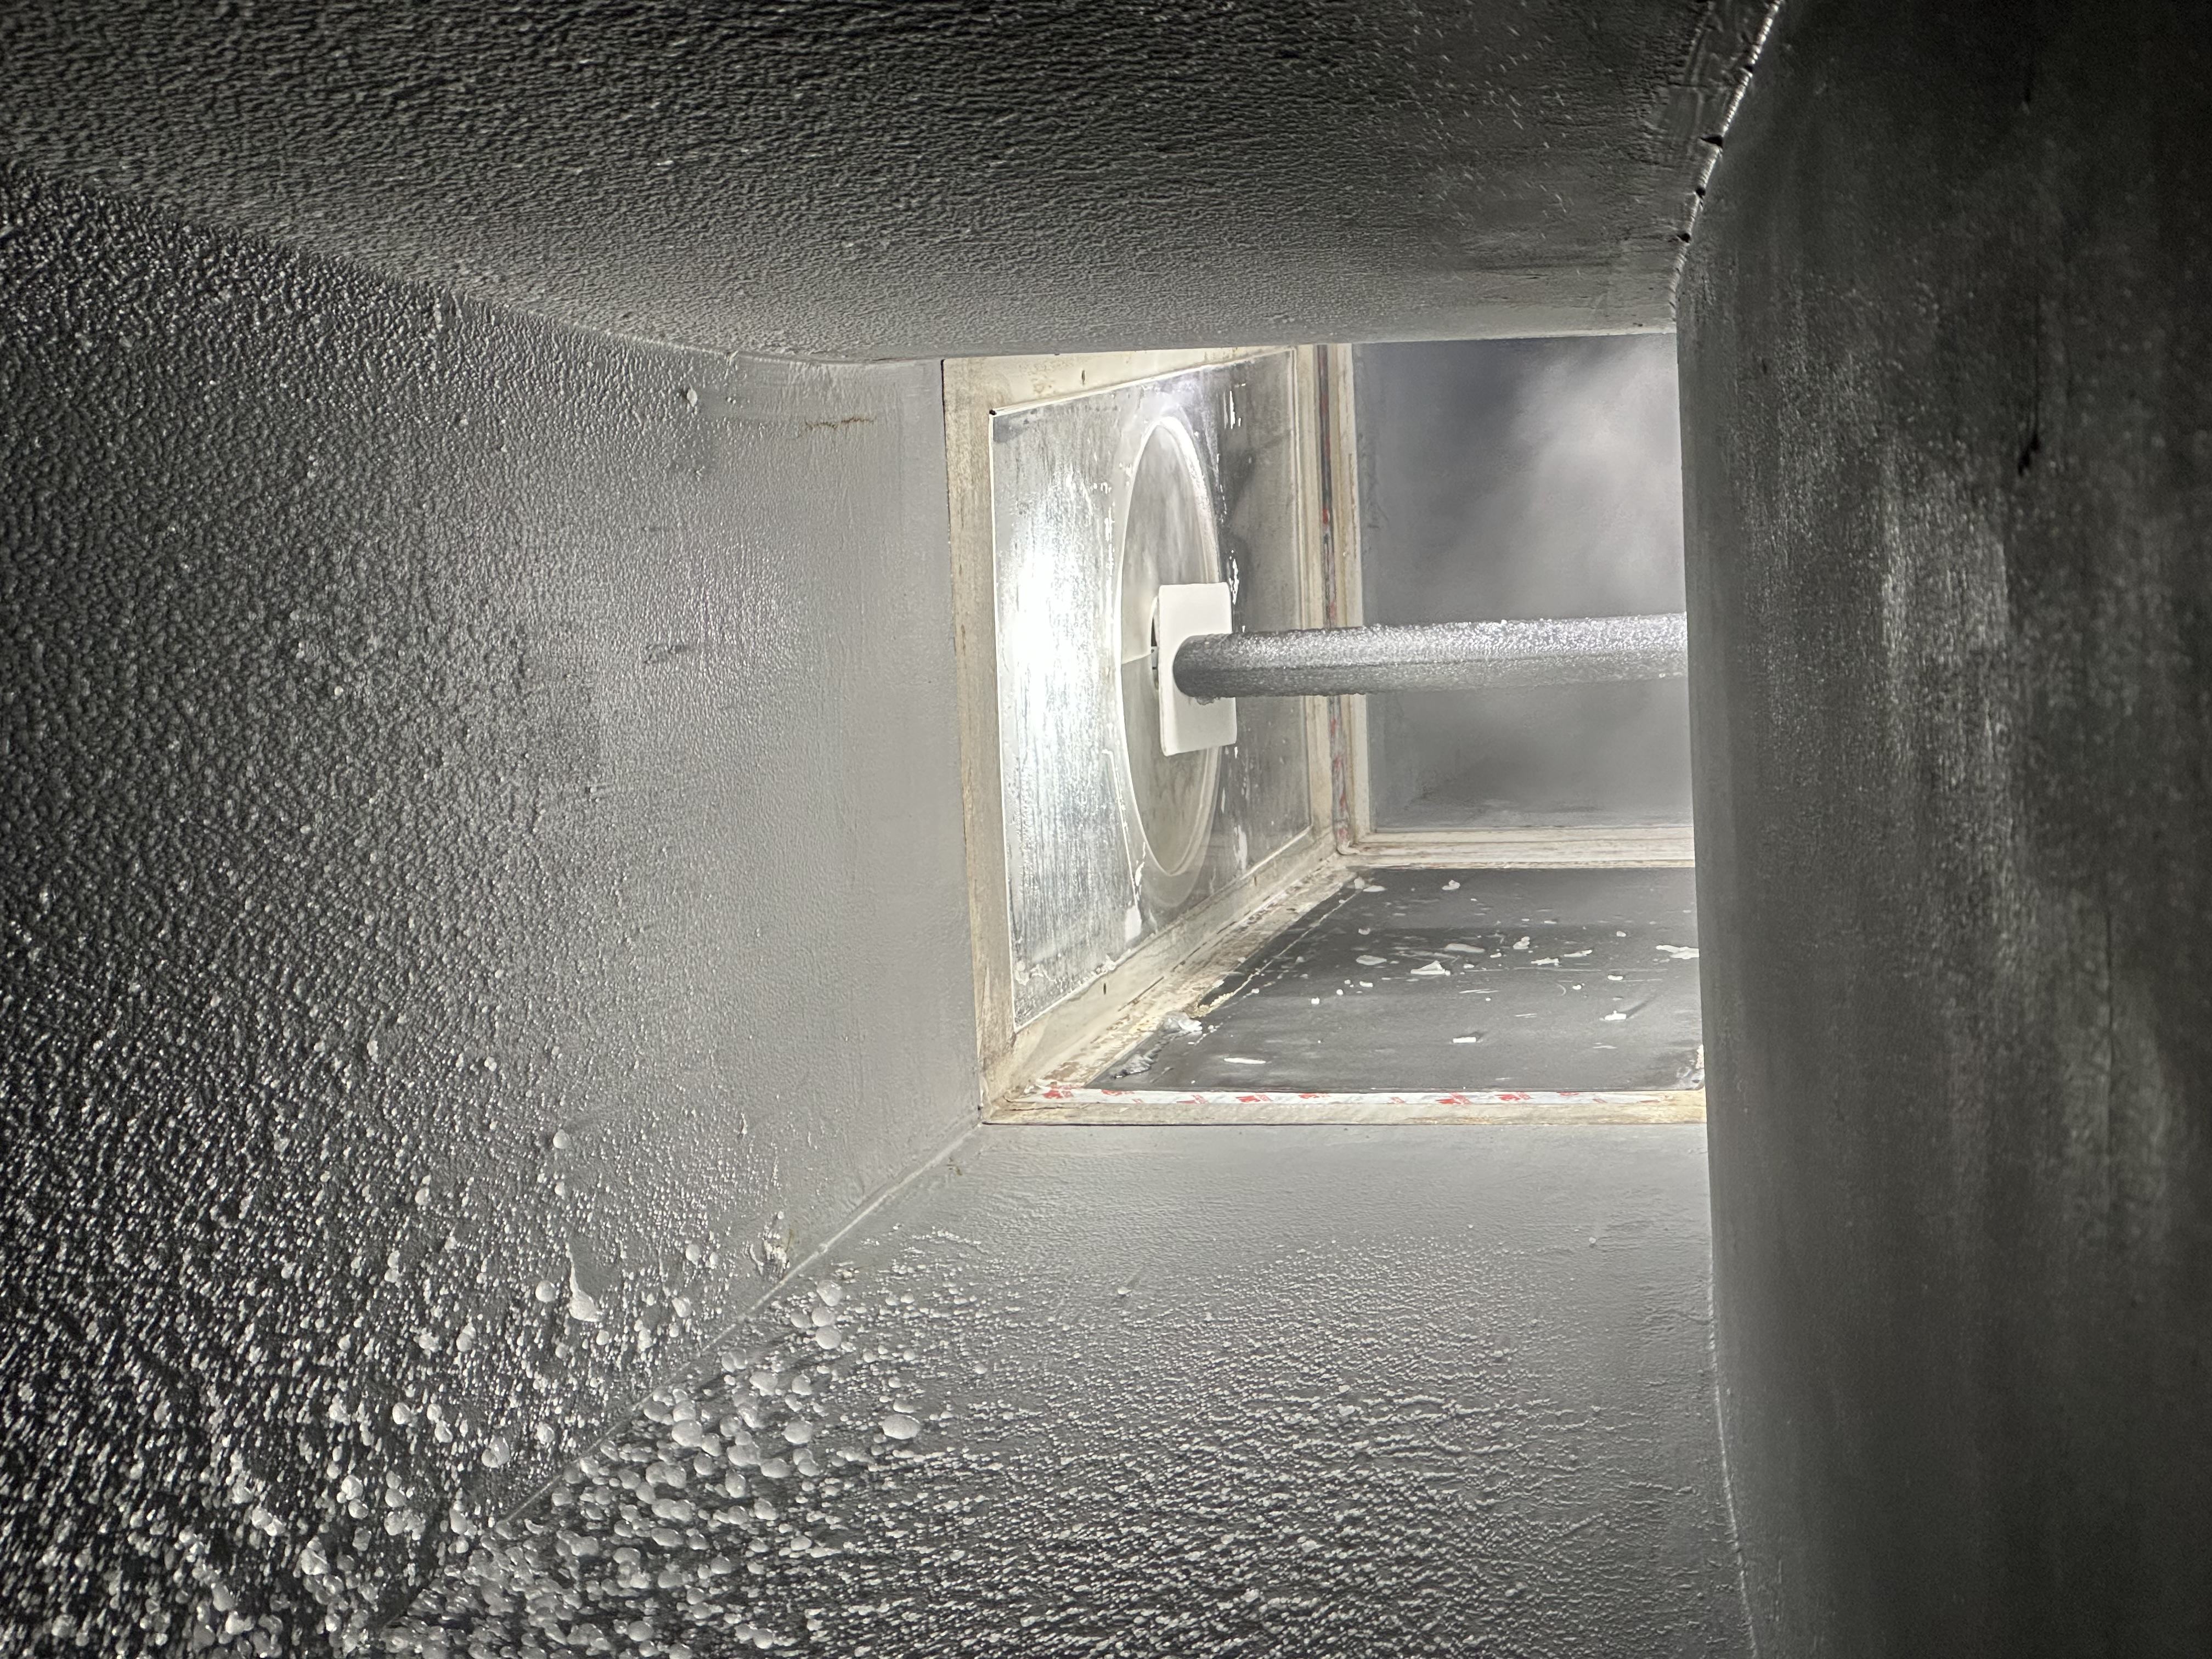
\includegraphics[width=\linewidth]{Figures/IMG_0230.jpeg}
    \caption{Start of the test section.}
    \label{fig:start_test_section}
\end{figure}

\newpage

\section{Full Size Figures} \label{sec:full_size_figures}

\begin{figure}[htpb]
    \centering
    \includesvg[width=\linewidth]{Figures/Coefficient of Lift vs. Angle of Attack.svg}
    \caption{Full size graph of the coefficient of lift versus the angle of attack.}
    \label{fig:full_c_l_vs_alpha}
\end{figure}

\begin{figure}[htpb]
    \centering
    \includesvg[width=\linewidth]{Figures/Coefficient of Drag vs. Angle of Attack.svg}
    \caption{Full size graph of the coefficient of drag versus the angle of attack.}
    \label{fig:full_c_d_vs_alpha}
\end{figure}

\begin{figure}[htpb]
    \centering
    \includesvg[width=\linewidth]{Figures/Coefficient of Moment vs. Angle of Attack.svg}
    \caption{Full size graph of the coefficient of moment versus the angle of attack.}
    \label{fig:full_c_m_vs_alpha}
\end{figure}

\begin{figure}[htpb]
    \centering
    \includesvg[width=\linewidth]{Figures/Lift to Drag Ratio vs. Angle of Attack.svg}
    \caption{Full size graph of the lift to drag ratio versus the angle of attack.}
    \label{fig:full_c_lbyc_d_vs_alpha}
    \vspace*{4.5in}
\end{figure}



